\documentclass[12pt,a4paper]{article}

\usepackage[utf8]{inputenc}
\usepackage{amsmath, array, geometry, enumitem, multicol, caption, booktabs}
\usepackage{float, babel, tabularx, booktabs, inconsolata, graphicx}
\usepackage[T1]{fontenc}
\geometry{margin=2.5cm}

\title{\textbf{Práctica 1. Clusters, funciones lógicas, código binario y código hexadecimal}}

\begin{document}

\date{\today}

\thispagestyle{empty}
\begin{figure}[ht]
	\minipage{0.75\textwidth}
	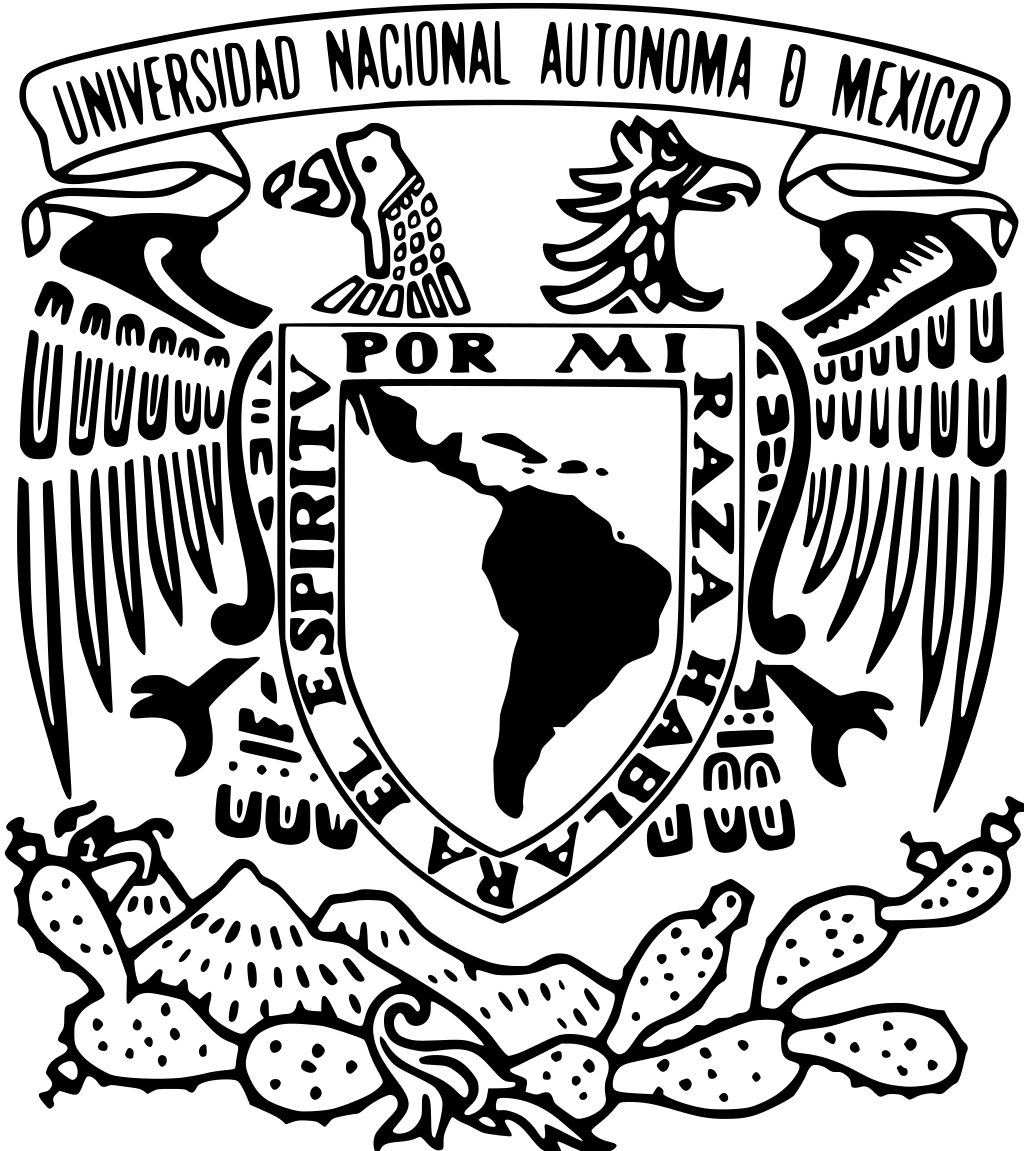
\includegraphics[width = 4.6 cm]{logo_unam.png}
	\endminipage
	\minipage{0.32\textwidth}
	
\includegraphics[height = 4.6cm, width = 4cm]{EscudoIIMAS.png}
	\endminipage
\end{figure}

\begin{center}
	\vspace{0.5cm}
	\LARGE
	UNIVERSIDAD NACIONAL AUTÓNOMA DE MÉXICO

	\vspace{0.5cm}
	\LARGE
	Instituto de Investigaciones en Matemáticas Aplicadas y Sistemas

	\vspace{1.2cm}
	\Large
	\textbf{Práctica 1. Clusters, funciones lógicas, código binario y código hexadecimal.}

	\vspace{1cm}
	\normalsize
	PRESENTA \\
	\vspace{.3cm}
	\large
	\textbf{\textit{Equipo 5} \\}
        \textbf{Esquivel Palacios Leonardo de Jesus\\}
        \textbf{Esteva Gallegos Carlos Fabián \\}
	\textbf{López Gónzalez Andrés\\}
        \textbf{Munive Ramírez Ibrahim\\}
	\textbf{Pérez Aguiar Oropeza Gabriel Emiliano\\}
	\textbf{Ríos Pérez Fany\\}    

	\vspace{1cm}
	\normalsize
	PROFESOR \\
	\vspace{.3cm}
	\large
	\textbf{Esp. Adrián Durán Chavesti}

	\vspace{1cm}
	\normalsize
	ASIGNATURA \\
	\vspace{.3cm}
	\large
	\textbf{Cómputo Concurrente}

	\vspace{1cm}
\end{center}

\newpage


\section*{Objetivos}
\begin{itemize}[label=--]
    \item Comparar las especificaciones más importantes de las computadoras más rápidas del mundo.
    \item Repaso de funciones lógicas básicas.
    \item Repaso de código binario y código hexadecimal.
\end{itemize}

\section*{Instrucciones}

\section{¿Qué es un cluster de servidores?}
Es un conjunto de servidores interconectados que trabajan juntos como si fueran uno solo, 
para aumentar la disponibilidad, el rendimiento y la fiabilidad de las aplicaciones y servicios.


\section{Áreas principales de uso de los clusters}
%\begin{multicols}{2}
\begin{enumerate}
    \item Milicia
    \item Predicción de clima
    \item Óptica
    \item Petrofísica
    \item Matemáticas
    \item Mecánica
    \item Química
    \item Ultrasonido
\end{enumerate}
%\end{multicols}


\section{Características principales del quinto computador más poderoso del mundo}

\begin{tabularx}{\textwidth}{>{\bfseries}l X}
\toprule
Nombre & Eagle - Microsoft NDv5, Xeon Platinum 8480C 48C 2GHz, NVIDIA H100, NVIDIA InfiniBand NDR \\
\midrule
País de origen & Estados Unidos de América \\
Nodos & 1,800 nodos Azure ND H100 v5 \\
Procesadores & Xeon Platinum 8480C 48C 2GHz \\
Memoria RAM & No hay información pública exacta. Se estima entre 384 GB y 15,200 GiB, según la serie de Azure utilizada. \\
Almacenamiento & Estimado: entre 4000 MBps y 8000 MBps, según la serie de Azure. \\
Redes & InfiniBand NDR, 400 Gbps \\
FLOPS & 561.20 PetaFlop/s \\
Sistema operativo & Ubuntu 22.04 \\
Principal uso & Desarrollo científico, ingenieril, backend de Azure e Inteligencia Artificial. \\
\bottomrule
\end{tabularx}

\section{Tablas de verdad}
\subsection{Escribir las tablas de verdad de las funciones lógicas siguientes:} 
and, xor, or, xnor, nand, not y nor.

\begin{multicols}{4}

% --- AND ---
\subsection*{AND}
\begin{tabular}{c c | c}
\toprule
A & B & X \\
\midrule
0 & 0 & 0 \\
0 & 1 & 0 \\
1 & 0 & 0 \\
1 & 1 & 1 \\
\bottomrule
\end{tabular}

% --- XOR ---
\subsection*{XOR}
\begin{tabular}{c c | c}
\toprule
A & B & X \\
\midrule
0 & 0 & 0 \\
0 & 1 & 1 \\
1 & 0 & 1 \\
1 & 1 & 0 \\
\bottomrule
\end{tabular}

% --- OR ---
\subsection*{OR}
\begin{tabular}{c c | c}
\toprule
A & B & X \\
\midrule
0 & 0 & 0 \\
0 & 1 & 1 \\
1 & 0 & 1 \\
1 & 1 & 1 \\
\bottomrule
\end{tabular}

% --- XNOR ---
\subsection*{XNOR}
\begin{tabular}{c c | c}
\toprule
A & B & X \\
\midrule
0 & 0 & 1 \\
0 & 1 & 0 \\
1 & 0 & 0 \\
1 & 1 & 1 \\
\bottomrule
\end{tabular}

% --- NAND ---
\subsection*{NAND}
\begin{tabular}{c c | c}
\toprule
A & B & X \\
\midrule
0 & 0 & 1 \\
0 & 1 & 1 \\
1 & 0 & 1 \\
1 & 1 & 0 \\
\bottomrule
\end{tabular}

% --- NOT ---
\subsection*{NOT}
\begin{tabular}{c | c}
\toprule
A & X \\
\midrule
0 & 1 \\
1 & 0 \\
\bottomrule
\end{tabular}

% --- NOR ---
\subsection*{NOR}
\begin{tabular}{c c | c}
\toprule
A & B & X \\
\midrule
0 & 0 & 1 \\
0 & 1 & 0 \\
1 & 0 & 0 \\
1 & 1 & 0 \\
\bottomrule
\end{tabular}

\end{multicols} 

\begin{verbatim}
       |\      _,,,---,,_
ZZZzz /,`.-'`'    -.  ;-;;,_
     |,4-  ) )-,_. ,\ (  `'-'
    '---''(_/--'  `-'\_)
\end{verbatim}

\subsection{Escribir la tabla de verdad del siguiente diagrama de compuertas lógicas:}

\begin{figure}[H]
    \centering
    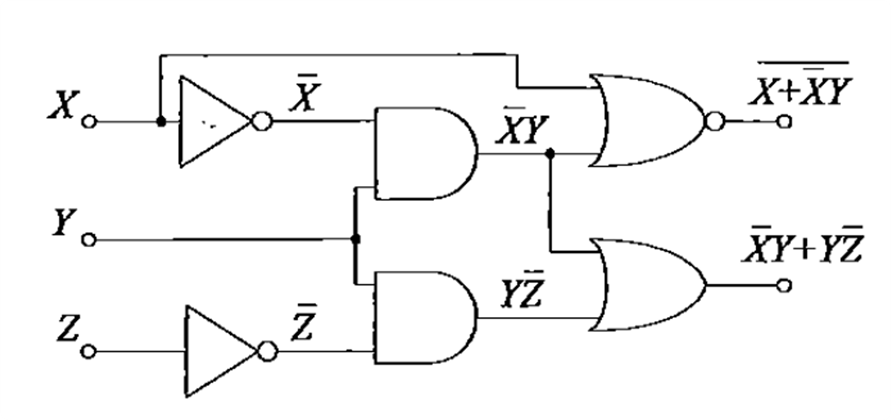
\includegraphics[width=0.5\linewidth]{Puertas lógicas.png}
    \caption{Diagrama de compuertas lógicas}
    \label{fig:puertas}
\end{figure}

\begin{table}[h]
\centering
\begin{tabular}{c c c | c | c }
\toprule
X & Y & Z & $\overline{ X + \overline{X}Y}$ & $\overline{X}Y + Y \overline{Z} $ \\
\midrule
0 & 0 & 0 & 1 & 0 \\
0 & 0 & 1 & 1 & 0 \\
0 & 1 & 0 & 0 & 1 \\
0 & 1 & 1 & 0 & 1 \\
1 & 0 & 0 & 0 & 0 \\
1 & 0 & 1 & 0 & 0 \\
1 & 1 & 0 & 0 & 1 \\
1 & 1 & 1 & 0 & 0 \\
\bottomrule
\end{tabular}
\end{table}

\subsection{Llenar la siguiente tabla según corresponda.}

\begin{table}[h]
\centering
\begin{tabular}{| c | c | c |}
\toprule
Decimal & Binario & Hexadecimal \\
\midrule
\textbf{1230} & \textbf{0100 1100 1110} & \textbf{4CE} \\
1433 & \textbf{0101 1001 1001} & 599 \\
1532 & 0101 1111 1100 & \textbf{5FC} \\
\textbf{1141} & 0100 0111 0101 & 475 \\
3864 & \textbf{1111 0001 1000} & F18 \\
3770 & 1110 1011 1010 & \textbf{EBA} \\
\textbf{1023} & 0011 1111 1111 & 3FF \\
352 & \textbf{0001 0110 0000} & 160 \\
2582 & 1010 0001 0110 & \textbf{A16} \\

\bottomrule
\end{tabular}
\end{table}

\newpage

\subsection*{Conversiones de Decimal a Binario y Hexadecimal}

\subsubsection*{1. Decimal: 1230}

\textbf{Decimal $\to$ Binario:}

\[
\begin{array}{c|c|c}
\text{División} & \text{Cociente} & \text{Resto} \\
\hline
1230 \div 2 & 615 & 0 \\
615 \div 2 & 307 & 1 \\
307 \div 2 & 153 & 1 \\
153 \div 2 & 76 & 1 \\
76 \div 2 & 38 & 0 \\
38 \div 2 & 19 & 0 \\
19 \div 2 & 9 & 1 \\
9 \div 2 & 4 & 1 \\
4 \div 2 & 2 & 0 \\
2 \div 2 & 1 & 0 \\
1 \div 2 & 0 & 1 \\
\end{array}
\]

\[
\text{Binario: } 0100\,1100\,1110
\]

\textbf{Binario $\to$ Hexadecimal:}

0100 = 4

1100 = C

1110 = E

\[
\text{Hexadecimal: } 4CE
\]

\subsubsection*{2. Binario: 0101 1001 1001}

\textbf{Binario $\to$ Decimal:}

\[
1\cdot2^0+0\cdot2^1+0\cdot2^2+1\cdot2^3+ 1\cdot2^4+0\cdot2^5+0\cdot2^6+1\cdot2^7 +1\cdot2^8+0\cdot2^9+1\cdot2^{10}+0\cdot2^{11} 
\]

\[
 = 2^0 + 2^3 + 2^4 + 2^7 + 2^8+2^{10}
\]

\[
 = 1 + 8 + 16 + 128 + 256 + 1024 
\]

\[
 = 153 + 1280  
\]

\[
 = 1433  
\]

\[
\text{Decimal: } 1433
\]

\textbf{Binario $\to$ Hexadecimal:}

0101 = 5

1001 = 9

1001 = 9

\[
\text{Hexadecimal: } 599
\]

\subsubsection*{3. Hexadecimal: 5FC}

\textbf{Hexadecimal $\to$ Binario:}

5 = 0101

F = 1111

C = 1100

\[
\text{Binario: } 0101\,1111\,1100
\]

\textbf{Binario $\to$ Decimal:}

\[
 = 0\cdot 2^0 + 0\cdot 2^1 + 1\cdot 2^2 + 1\cdot 2^3
 + 1\cdot 2^4 + 1\cdot 2^5 + 1\cdot 2^6 + 1\cdot 2^7
 + 1\cdot 2^8 + 0\cdot 2^9 + 1\cdot 2^{10} + 0\cdot 2^{11}
\]

\[
 = 2^2 + 2^3 + 2^4 + 2^5 + 2^6 + 2^7 + 2^8 + 2^{10}
\]

\[
 = 4 + 8 + 16 + 32 + 64 + 128 + 256 + 1024 
\]

\[
\text{Decimal: }  1532
\]

\subsection{Referencias}

NREL – Eagle Supercomputer
National Renewable Energy Laboratory. (2019, January 8). NREL’s New Supercomputer, 
Eagle, Takes Flight. National Renewable Energy Laboratory. 
 
 https://www.nrel.gov/manufacturing/news/program/2019/nrel-new-supercomputer-eagle-takes-flight#:~:text=Now%20in%20production%20use%2C%20the,accelerate%20our%20energy%20system%20transformation www2.nrel.gov

\noindent\rule{\textwidth}{0.4pt}

Top500 – June 2025 List
TOP500. (2025, junio). TOP500 Supercomputer Sites – June 2025. TOP500. 
 
https://top500.org/lists/top500/2025/06/ top500.org

\noindent\rule{\textwidth}{0.4pt}

Glenn Klockwood – Eagle (Microsoft)
Klockwood, G. (s. f.). Eagle (Microsoft). In The HPC Gardener. 
 
https://glennklockwood.com/garden/systems/Eagle glennklockwood.com

\noindent\rule{\textwidth}{0.4pt}

Glenn Klockwood – Azure ND H100 v5 Node
Klockwood, G. (s. f.). Azure ND H100 v5. In The HPC Gardener. 
 
https://glennklockwood.com/garden/nodes/Azure-ND-H100-v5 glennklockwood.com

\noindent\rule{\textwidth}{0.4pt}

Microsoft Learn – Dasv6 Series
Microsoft Corporation. (2024, noviembre 21). Dasv6 sizes series. Microsoft Learn. 
 
https://learn.microsoft.com/en-us/azure/virtual-machines/sizes/general-purpose/dasv6-series?tabs=sizebasic Microsoft Learn

\noindent\rule{\textwidth}{0.4pt}

Microsoft Learn – Msv2 Medium Memory Series
Microsoft Corporation. (2025, junio 6). Msv2 Medium Memory size series. Microsoft Learn. 
 
https://learn.microsoft.com/en-us/azure/virtual-machines/sizes/memory-optimized/msv2-mm-series?tabs=sizebasic Microsoft Learn

\noindent\rule{\textwidth}{0.4pt}

Microsoft Learn – Msv3 High Memory Series
Microsoft Corporation. (2025, junio 6). Msv3 High Memory size series. Microsoft Learn. 

https://learn.microsoft.com/en-us/azure/virtual-machines/sizes/memory-optimized/msv3-hm-series?tabs=sizebasic Microsoft Learn
 

\end{document}
